\documentclass[sigconf]{acmart}

\settopmatter{printacmref=false} % Removes citation information below abstract
\renewcommand\footnotetextcopyrightpermission[1]{} % removes footnote with conference information in first column
\pagestyle{plain} % removes running headers

\usepackage{booktabs} % For formal tables
% \usepackage[utf8]{inputenc}    
% \usepackage[T1]{fontenc}
\usepackage{graphicx}
% \usepackage{url}
% \usepackage[breaklinks]{hyperref}

% \usepackage{multirow}


\DeclareUnicodeCharacter{00A0}{ }

% Copyright
%\setcopyright{none}
%\setcopyright{acmcopyright}
%\setcopyright{acmlicensed}
\setcopyright{rightsretained}
%\setcopyright{usgov}
%\setcopyright{usgovmixed}
%\setcopyright{cagov}
%\setcopyright{cagovmixed}
\usepackage{graphicx}

% \copyrightyear{2017}


% \acmArticle{4}
% \acmPrice{15.00}


\begin{document}
\title{A Chance to Work}
\subtitle{Understanding the composition of foreign workers 
pursuing \\specialty occupations on the United States H-1B visa
}


\author{\textbf{Alexander Buddenbaum}}
\affiliation{%
  \institution{Georgia Institute of Technology}
%   \streetaddress{North Avenue}
  \city{Shenzhen} 
  \country{China}
}
\email{alex.budd@gatech.edu}

\author{\textbf{Qinrui Li}}
\affiliation{%
  \institution{Georgia Institute of Technology}
%   \streetaddress{North Avenue}
  \city{Shenzhen} 
  \country{China} 
}
\email{qli449@gatech.edu}

\author{\textbf{Tianyu Li}}
\affiliation{%
  \institution{Georgia Institute of Technology}
%   \streetaddress{North Avenue}
  \city{Shenzhen} 
  \country{China}  
}
\email{tli303@gatech.edu}


\author{\textbf{Chuanqi Liu}}
\affiliation{%
  \institution{Georgia Institute of Technology}
%   \streetaddress{North Avenue}
  \city{Shenzhen} 
  \country{China}
}
\email{cliu732@gatech.edu}

\author{\textbf{Tianshu Tao}}
\affiliation{%
  \institution{Georgia Institute of Technology}
%   \streetaddress{North Avenue}
  \city{Shenzhen} 
  \country{China} 
}
\email{ttao35@gatech.edu}



\maketitle
\pagestyle{plain}
\section{Introduction}


The United States Person in Specialty Occupation Visa, more commonly known as the H-1B visa, 
allows employers in the United States to hire temporary foreign workers specializing in one of many key occupations.  
Although a popular visa among college graduates aspiring to work in the United States, 
with a well-documented application process, 
there remains significant student interest in understanding the typical profile of successful 
H-1B visa applicants. 
To date, numerous studies have been conducted on recent years’ certification 
data in an attempt to analyze hiring trends. 
However, the usefulness of these studies remains to be questioned as they 
generally lack interactive visualizations for the user to gain 
insight from this information. In this study, we seek to understand recent 
hiring trends among US employers as well as the makeup of 
applications for these roles to project economic sectors with growth potential, 
creating meaningful visualizations for potential work 
visa applicants to interpret current data, and predict the outcome of future applications 
in an attempt to help international students make more informed career planning 
decisions when looking to work in the US.


\section{Related work}


As annual H-1B application records are publicly available through the US Department of Labor, 
this data has been a popular topic for machine learning researchers as well as online enthusiasts.  
The topic has also inspired several versions of truncated datasets that have been aggregated by several websites as a resource 
for international applicants, and basic analyses appear frequently in academic journals. The general consensus among 
scholarly literature points to an overall positive economic impact by H-1B workers in the United States (Butler 2012, Peri 2014) and 
skilled immigrant workers successfully integrate into the general population (Grimm 2019, Hermansen 2022). 
Interestingly, none of these studies or websites have successfully integrated the database, 
visualizations, and prediction algorithms under one application. 



We have considered several methods for data cleaning and integration. H-1B application data from the US DOL total over 3 million 
records from 2017 to 2021. Chatterjee et al., use Python packages Pandas and Numpy for data cleansing, including the 
completion of incomplete data in H-1B application data, column name renaming and subset selection (Chatterjee 2021). Specific operations can be done 
by calling Python packages. Looking closely at their data, however, we found that not only is it from a non-official and unverifiable 
source; their records are also severely truncated, and did not effectively consolidate job titles with negligible spelling variations. 
Perhaps this truncation and lack of cleansing was out of convenience, but unfortunately this was the case for the majority of studies 
we read during preliminary research. As the datasets among the different years generally only differ by a few column names while 
retaining similar organization, we find it more convenient to use open-sourced applications such as OpenRefine to clean the data, selecting features 
that may be the most meaningful to the reader (Chadha 2021).  
Dombe et al. use SQLite for its lightweight data storage and access (Dombe 2020).  



Several online databases exist providing similar information. The most accurate and comprehensive websites include H-1B Grader and 
One Point Three Acres, which have aggregated US Department of Labor statistics into textual tables which allow for filtering based 
on attributes such as country of origin, job title, sponsoring employer, and salary band(1Point3Acres 2022, H1BGrader 2022). These are relatively complete 
relational database systems with interactive visualizations. The data is also collected directly from the US DOL and up to date. 
As the data provided by US DOL is in XLS format and consists of over 26 attributes in its initial form, the SQL-style database used 
by these websites appears most appropriate. However, these websites are unable to predict application outcomes for users, thus the 
users must perform their own extrapolations based on their subjective interpretations of recent trends.



Most academic studies rely on various Python libraries for visualizations. Tandon et al compares Python and Tableau as accessible technologies 
for quickly producing charts (Tandon 2021). A similar approach is taken by Chavda et al, analyzing records with Apache Hive and Pig with Tableau 
visualizations (Chavda 2019). We elected to use D3 in Javascript for its rich features and greater availability of documentation 
for creating interactive charts. 



The majority of the research to date compares the performance of several machine learning algorithms in predicting application outcomes. 
Random Forest appears to be the most popular model among other studies (Sundararaman 2017), but other methods have been tested as well. 
Swain et al. compared the accuracy of random forest, k-means clustering, and logistic regression algorithms for predicting 
H-1B application acceptance based on roughly 3 million data points from 2011 to 2016 (Swain 2018), and Chatterjee et al. propose an artificial 
neural network (Chatterjee 2021). They also show a variety of static charts, but the charts only compare across one dimension at a time. The data is 
also nearly ten years old. While these studies set us in a good direction for doing some basic analysis, we seek to augment them 
through an interactive visualization allowing the user to view results based on multiple attributes such as salary and location. 
Thakur et al apply seven classification models - Decision tree, C5.0, Random
Forest, Naïve Bayes, Neural Network and SVM - to predict the status of each H-1B application (Thakur 2018). 
Interestingly, their C5.0 decision tree model proved the most accurate on the same data set used by Swain et al in their research. 
Their liberal use of bar charts makes some of their findings hard to follow. Similar results were found by Jethwani et al, who 
achieved the highest prediction accuracy with a decision tree as opposed to random forest and logistic regression (Jethwani 2019). 
We will run a more recent data set to better reflect 
current trends, and instead of comparing several classifiers for their accuracy, we will focus more on providing meaningful insights 
to users through the dynamic integration of the charts.



The method espoused by Raunak Roy uses the collected feedback in applying the analytic hierarchy process and entropy 
weight method to evaluate the data analysis and prediction model (Roy 2021). This method decomposes the decision-making problem into different 
hierarchical structures according to the order of general objectives, sub objectives at all levels, evaluation criteria and specific 
standby choice. Then, the problem is reduced to the determination of the relatively important weight of the lowest level, such as 
schemes and measures for decision-making, relative to the highest level - the overall goal or the arrangement of the relative 
advantages and disadvantages, so as to judge whether the prediction scheme we provide can meet the needs of users on whether to 
apply for H-1B visa.


\section{Proposed method}


In order to show comprehensive aspects of H-1B statistics to potential users, we propose a set of interactive visualizations, 
employing multiple widely used D3.js charts implemented in Vue and Flask.  The data is publicly available, and all the tools 
are open source and can be deployed from a consumer-grade computer. As such, this project requires no special funding. 



We retrieve H-1B application data from years 2017 to 2021 from the US Department of Labor. All records from these five 
years in their original XLS format totaled over 1.5Gb. By accessing data directly from its original source, we can 
guarantee our data will have the highest possible integrity for more accurate evaluation and predictions. 
There are some inconsistencies in the naming and ordering of columns from year to year, as well as the addition of columns that are not pertinent to 
our analysis.  We use OpenRefine to clean and standardize the data, dropping columns that are not pertinent to our 
analysis, thus making the file sizes manageable before consolidating into CSV files aggregated by year. 
\begin{figure}
  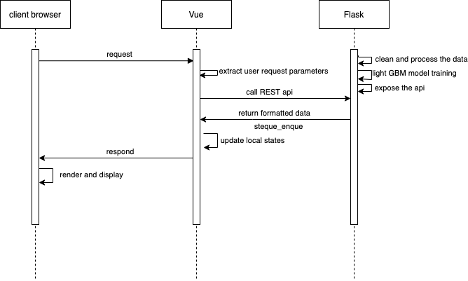
\includegraphics[width=\linewidth]{fig4.png}
  \caption{App Process Flow}
  \label{fig:appprocessflow}
\end{figure}

Users will select the attributes they are interested in on our portal page. Their request will be passed to our 
backend REST API, implemented by Python Flask. The API will then send the corresponding statistics back to the 
front-end interface. The user interface will then process the data and render the chart on the newly-directed page, 
where the user can view and interact with the chart using their cursor. The front-end application, based on Vue and D3.js, 
will have an interactive interface to provide the user rich choices of viewing, comparing, selecting and searching by certain fields. 



As mentioned in Related Work, other implementations exist on the Web. Our implementation is distinct from these earlier 
implementations by including several innovations or improvements. Our system provides users with more selections and 
chart types that are more relevant to the user, such as a US choropleth with state-by-state comparison. 
We provide more relevant details with the ability to combine search parameters such as state and salary. 
We also introduce H-1B application outcome prediction through machine learning methods, a feature we have yet to find on 
any frequently accessed website. A list of innovations and improvements is listed in Appendix B.  


We also construct a model that can predict the probability that a given application will be certified by the DOL. 
We drop unimportant features by the results of correlation and manual selection based on prior domain knowledge. 
We split the data 70\%-30\% for training and testing. 
We define our task as a binary classification, setting the “Certified” status as 1 and all other non-certified statuses 
as 0 to train our model. For the model, we choose a gradient boosting decision tree model named LightGBM because the data 
is nonlinear as we believe that this tree model shows improved performance over some of the commonly applied linear models. 
We cross-validate the data with 10 folds. 



\begin{figure}
  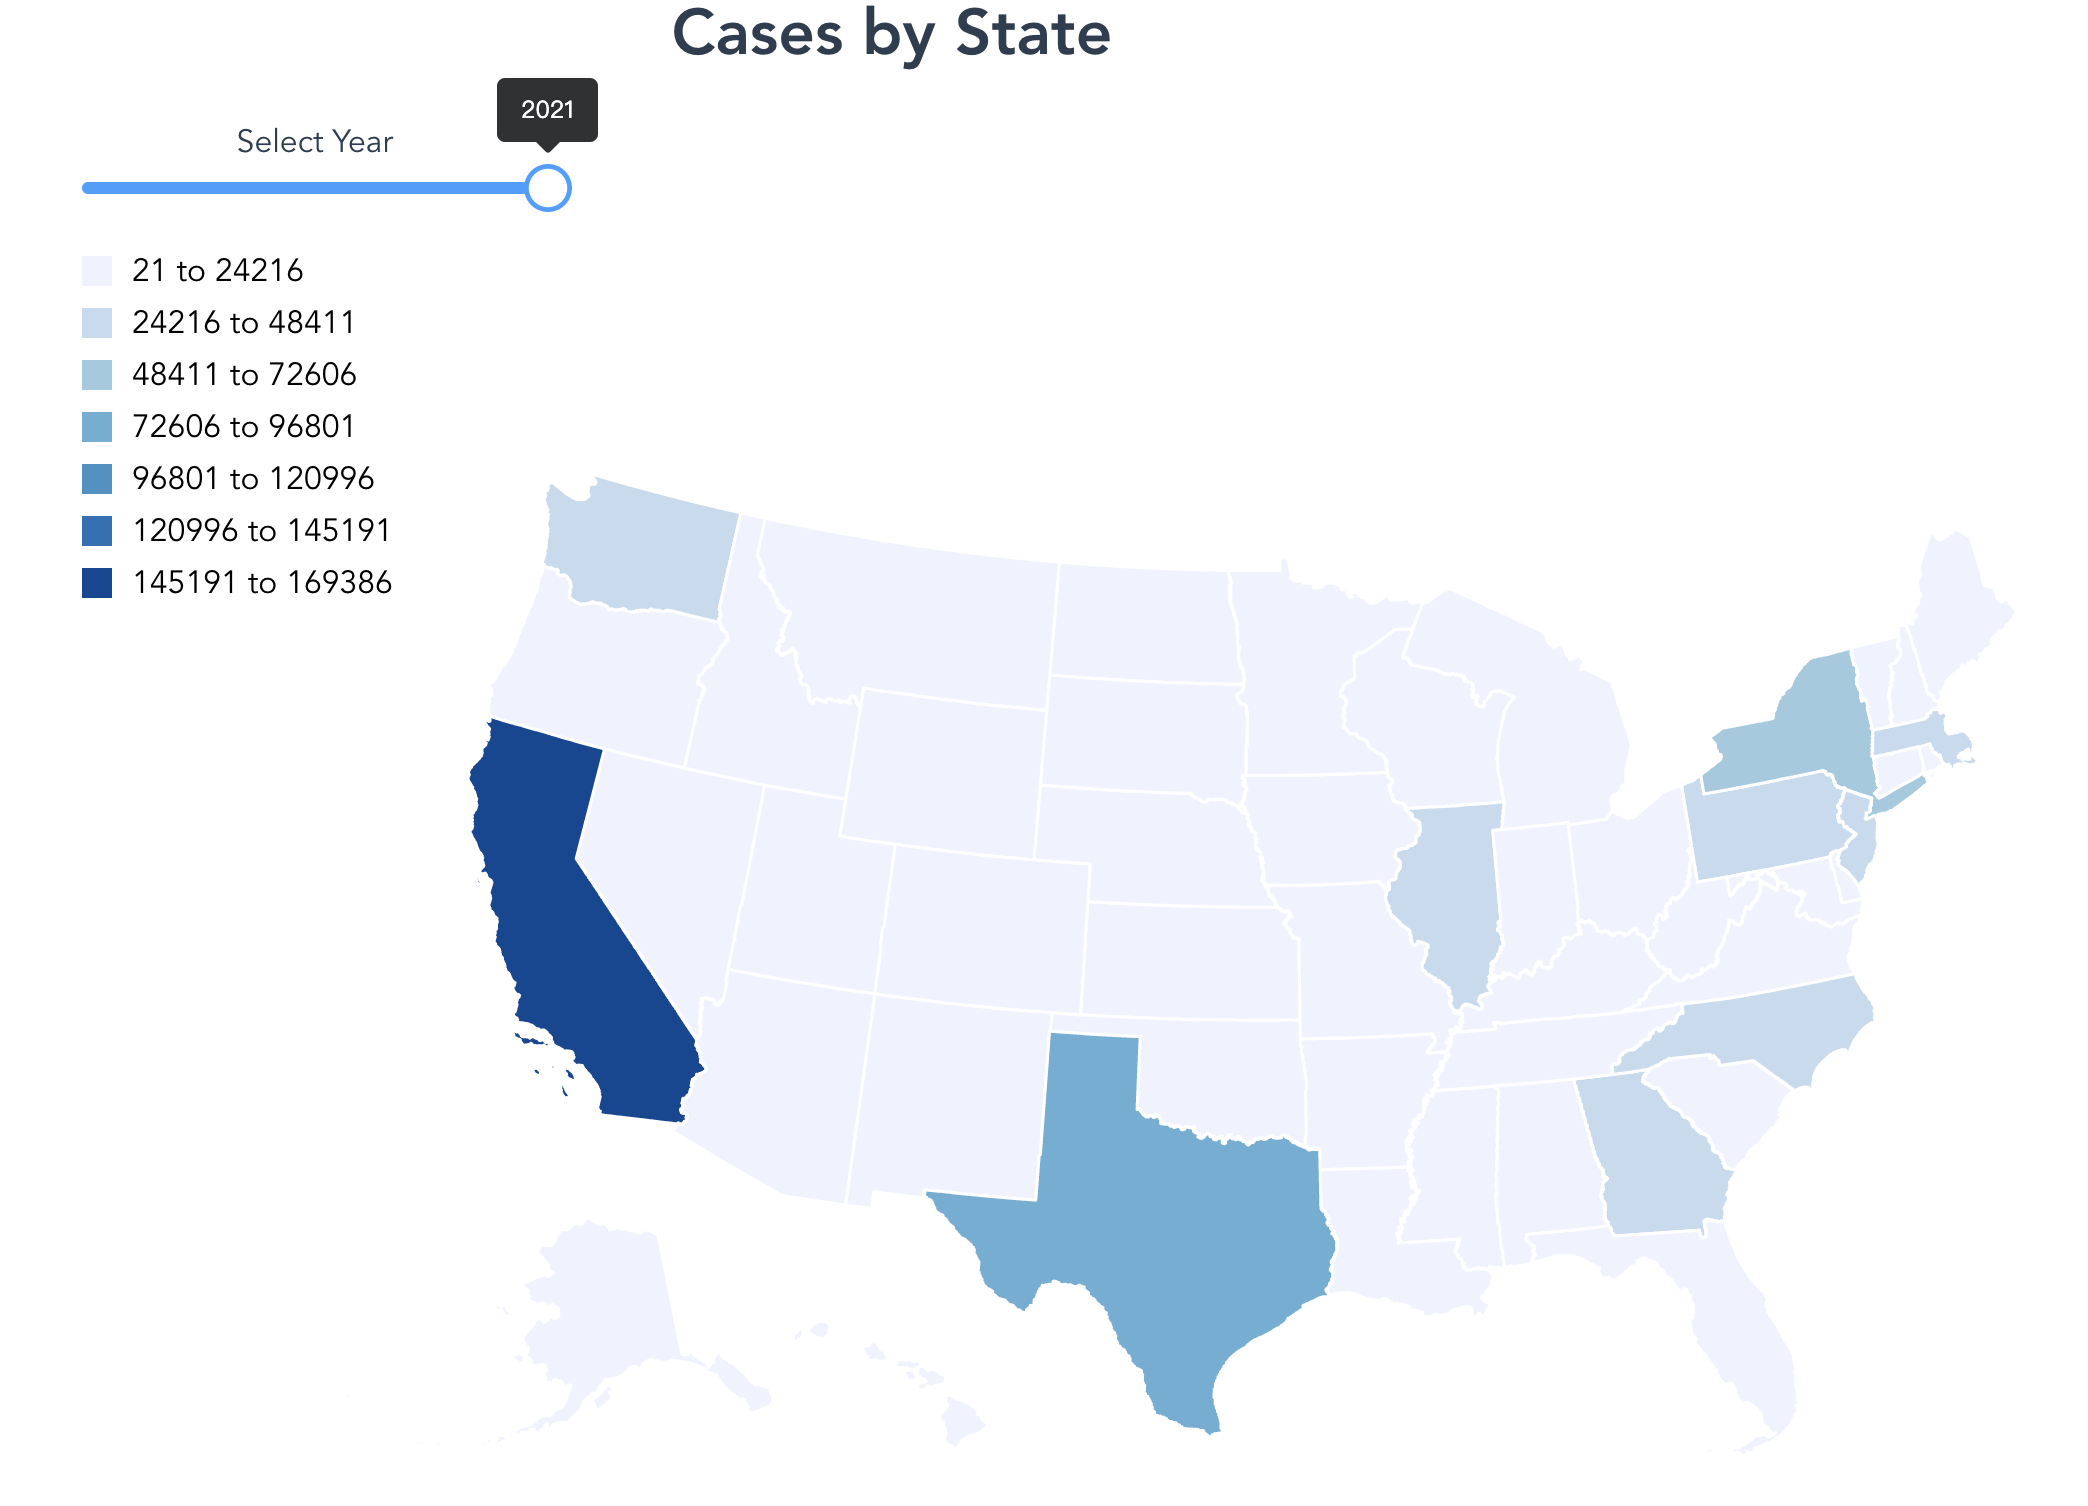
\includegraphics[width=\linewidth]{report_images/worksite2021.png}
  \caption{Top States by Application Count - 2021}
  \label{fig:topstates2021}
\end{figure}



\section{Experiments and Evaluation}

We have followed the original work distribution, which is distributed evenly among all 5 team members, 
with each member responsible for one component as well as making limited contributions to other components (see Appendix A). 


\subsection{Data Preprocessing and Feature Selection}

The raw data from US Department of Labor, organized by fiscal quarter, 
included as many as 30 attributes depending on the reporting year, 
making the data files quite cumbersome to manage. 
As several of our members are familiar with the H-1B application process, 
we were able to complete an initial manual feature selection with the assistance 
of the official US DOL documentation using OpenRefine, 
removing several attributes clearly irrelevant to our study. 
We retained the following attributes for our analysis:

  \begin{itemize}
    
  \item \textbf{Case number}: Unique identifier for each application record.
  \item \textbf{Case status}: Result of petition, 
  ie. Certified, Withdrawn, Denied. 
  \item \textbf{SOC code}: Official occupation title as defined by US Bureau of Labor Statistics, 
  ie. Software Developer, Computer Systems Analyst.
  \item \textbf{NAICS code}: Primary industry sector/vertical of employer as defined by 
  the North American Industry Classification System, 
  ie. Manufacturing, Information.
  \item \textbf{Full time position}: Whether the position is full-time.
  \item \textbf{Worksite state}: State of primary location of employment,
  ie. CA, NY, TX.
  \item \textbf{Worksite city}: City of primary location of employment, 
  ie. Menlo Park, Austin.
  \item \textbf{Employer name}: Name of petitioning employer,
  ie. Amazon, Deloitte.
  \item \textbf{Employer Business DBA}: Alternate name for employer. 
  \item \textbf{Total workers}: Number of workers included in a single petition. 
  Often the case when an employer hires several workers with the same occupation title. 
  \item \textbf{Wage rate of pay - From}: Minimum prevailing annual salary for the position.
  ie. \$85,000.
  \item \textbf{Wage - unit of pay}: Our analysis concentrates on USD paying occupations.

  \end{itemize}

A test run with the data using several gradient boosting decision tree learners, 
mentioned in more detail below, achieved an F1 score of 98\% on both testing 
and training data; therefore, we retained the exact attributes from our manual selection. 


We apply regular expressions to remove superfluous characters from the records, 
such as commas and dollar signs from some of the wage entries, 
as well as correct input errors and standardize capitalization of Case Status entries, 
and standardized Worksite State to display the full name of their respective states.  


The alpha iteration of our application revealed several glaring data quality issues that 
surprised us as this data comes directly from the US federal government. 
These were mostly input errors, such as incorrect capitalization, 
superfluous or missing punctuation and/or whitespace, 
numbers and special characters in alpha only fields, 
non-existent state names, state name included with city name, et cetera. 
This surprised us that data from the US federal government would be so dirty and lack validation. 
We then had to go back revise our cleansing suite to include more comprehensive operations using the 
Python library Pandas with regular expressions. 
Eventually, we dropped the SOC Name field altogether and replaced it with the SOC Code, which we 
then mapped to the SOC Name set provided by the US Bureau of Labor Statistics. Entries with 
an SOC Code not matching the official format made up less than 0.01\% of the total entries and thus 
were eliminated from our consideration. 

We also discovered several outliers with wages that are far beyond the typical range. 
We set an accepted wage ceiling at \$350,000 to mitigate any potential skewing of results 
by these outliers. 


\begin{figure}
  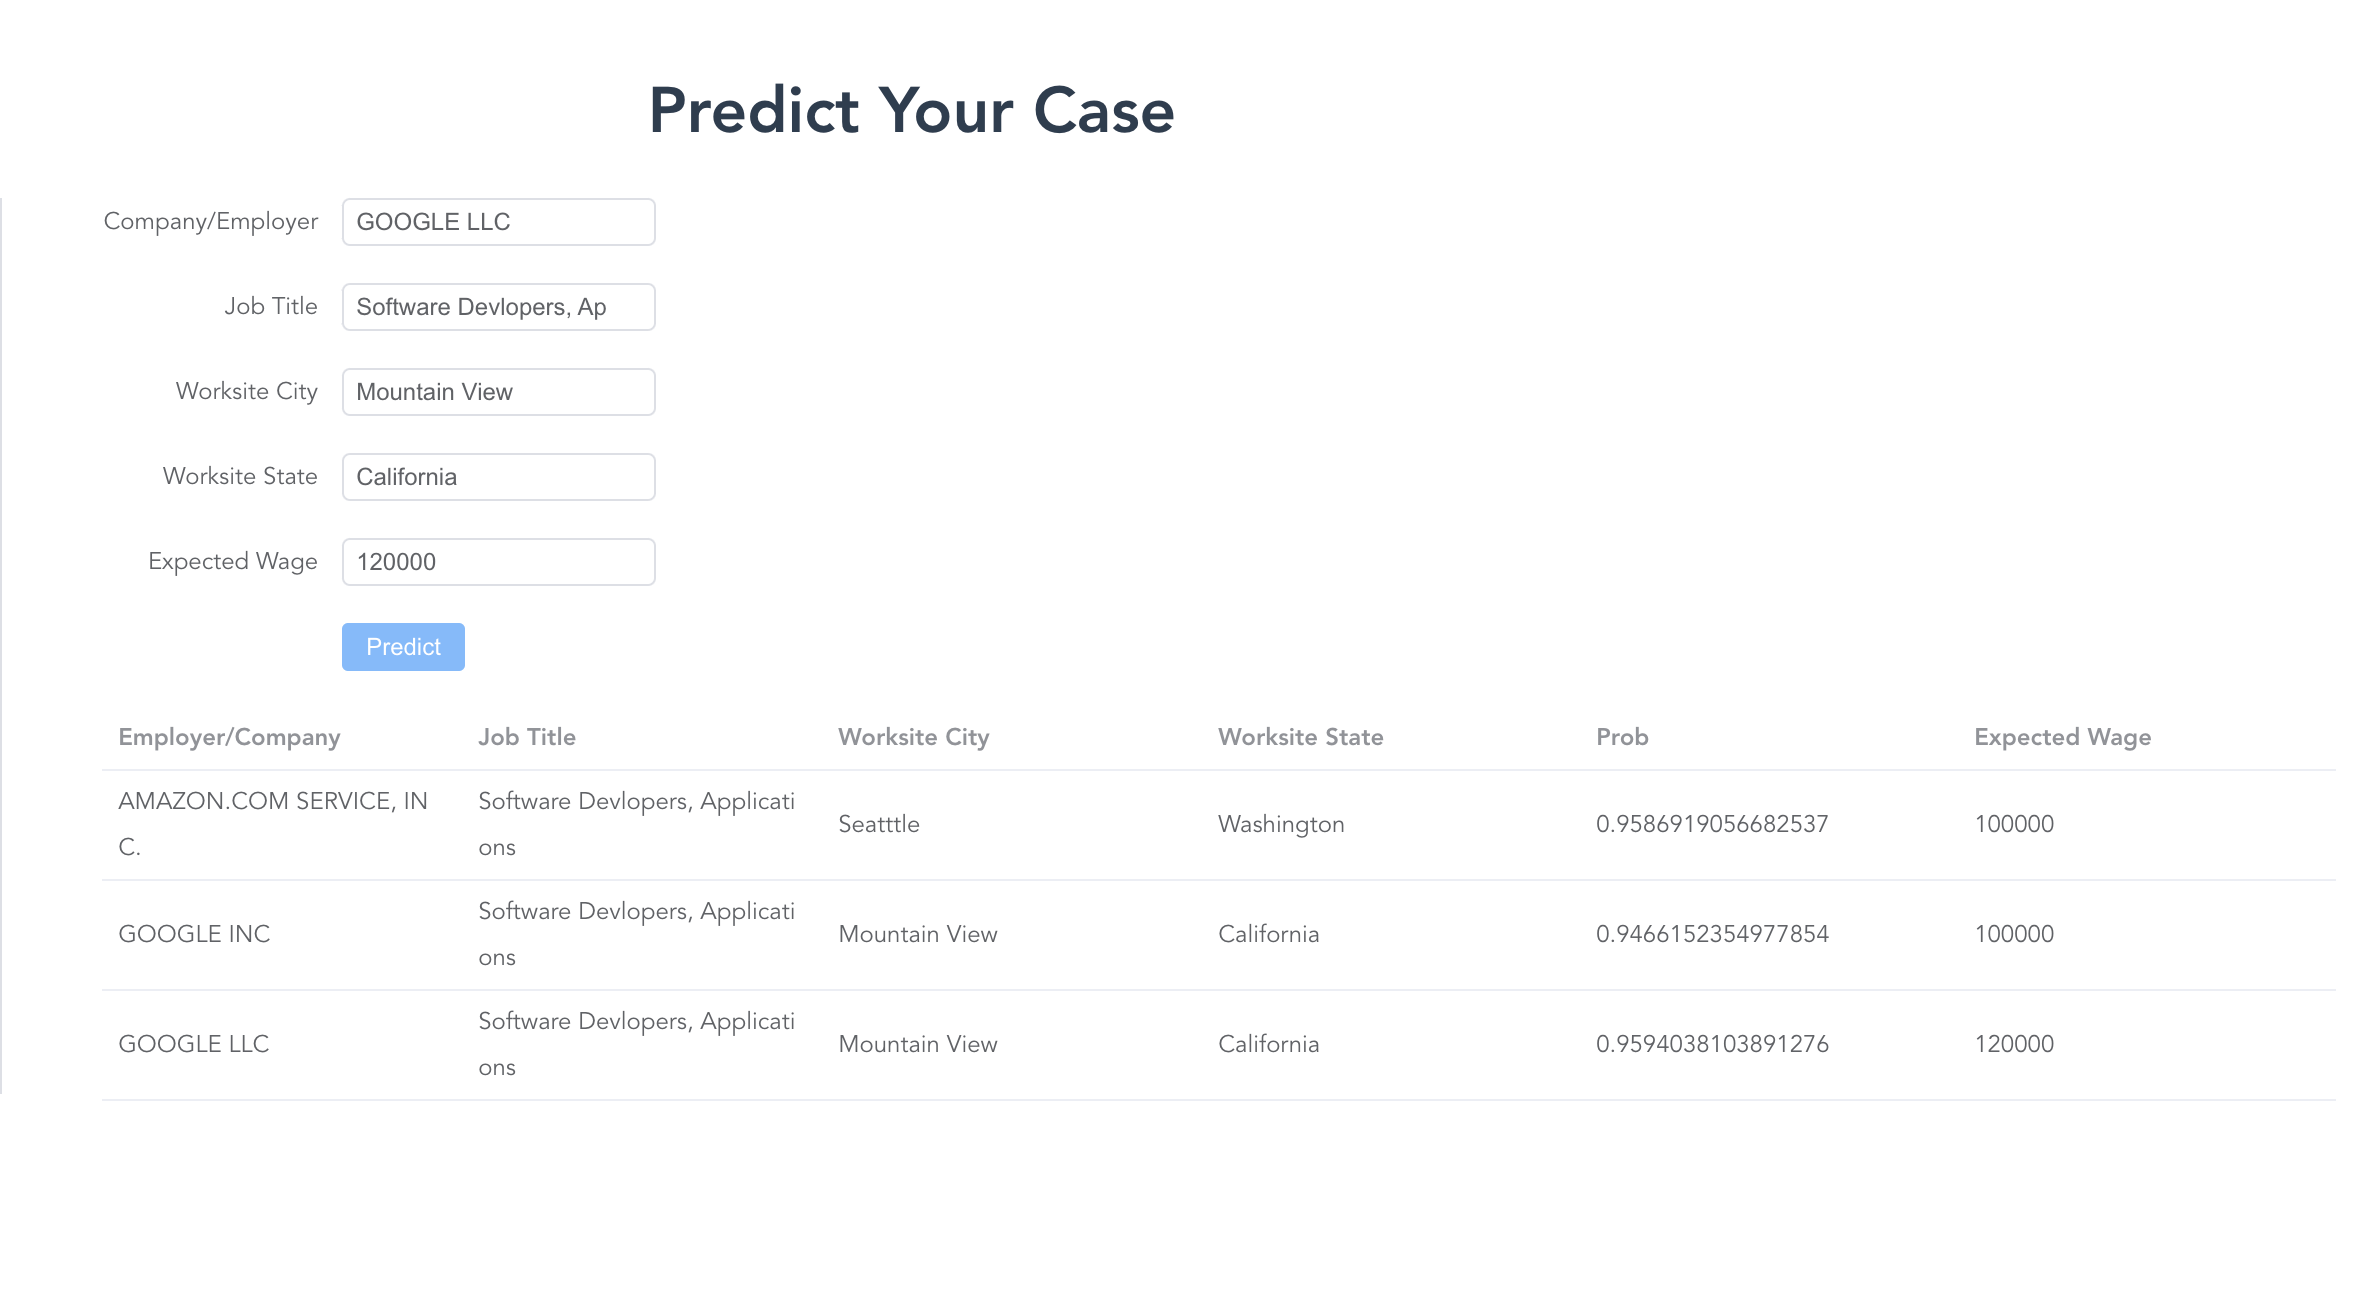
\includegraphics[width=\linewidth]{predict.png}
  \caption{Certification Prediction Interface}
  \label{fig:predict}
\end{figure}


\subsection{Prediction Algorithm}
Based on existing literature, various boosting decision tree models have generally proven 
the most accurate with historical application data due to the non-linear characteristics of the 
categorical data. 

We investigated several open-source gradient boosting frameworks, including XGBoost, 
Yandex’s CatBoost, and Microsoft’s LightGBM. We tested all three frameworks on 
all 5 years of data with a 30\%-70\% training split and 10-fold cross validation. 
While all provided very high accuracy and an F1 score of 97\%, 
our choice of LightGBM running 100 learners with 0.05 learning rate, unrestricted maximum depth, 
and the default number of leaves of 31, ran 20\% faster than the others. As are fairly satisfied 
with these results and declined to explore other models for this implementation.


\subsection{Visualization and Integration}
We integrated all visualizations and our predictor within a single 
web application built on the Flask framework, with a responsive interface using Vue, so that 
the user clicks a link to access one of several visualizations of any given year's applications 
by state, employer, or job title. The integration of all functionality under a single application 
turned out to be the most time-consuming part of our project, as individual components that worked 
flawlessly as standalone components would not always function properly on integration. 

We initially showed the total number of applications for each year in a bar chart, as well as a breakdown by application 
outcome as a line chart. We later consolidated this information into a stacked bar chart to show the trend in total number 
of applications as well as year-on-year differences for each different application outcome. 

We have a separate bar chart to represent the top ten employers with the greatest number of applications for each year. 
Earlier iterations showed that larger companies often apply using different subsidiaries with similar names, 
differentiated only by "Inc", "LLC", or other suffixes. We aggregated these more obvious employer name variations 
to make the comparisons more meaningful for the average user (potential job applicant). 

The top ten job titles (SOC names) for each year are also expressed with a bar chart. We avoided 
potential data inconsistencies in job titles by basing our comparison on the official job title provided 
by the US Department of Labor Statistics. 

We also provide the number of successful applications and their respective likelihood of certification 
by salary, by increments of \$25,000. The salary value for each sample is the greater value among 
the US DOL determined prevailing wage and the low end of the salary range offered for that position by 
its respective employer. 


% \begin{figure}
%   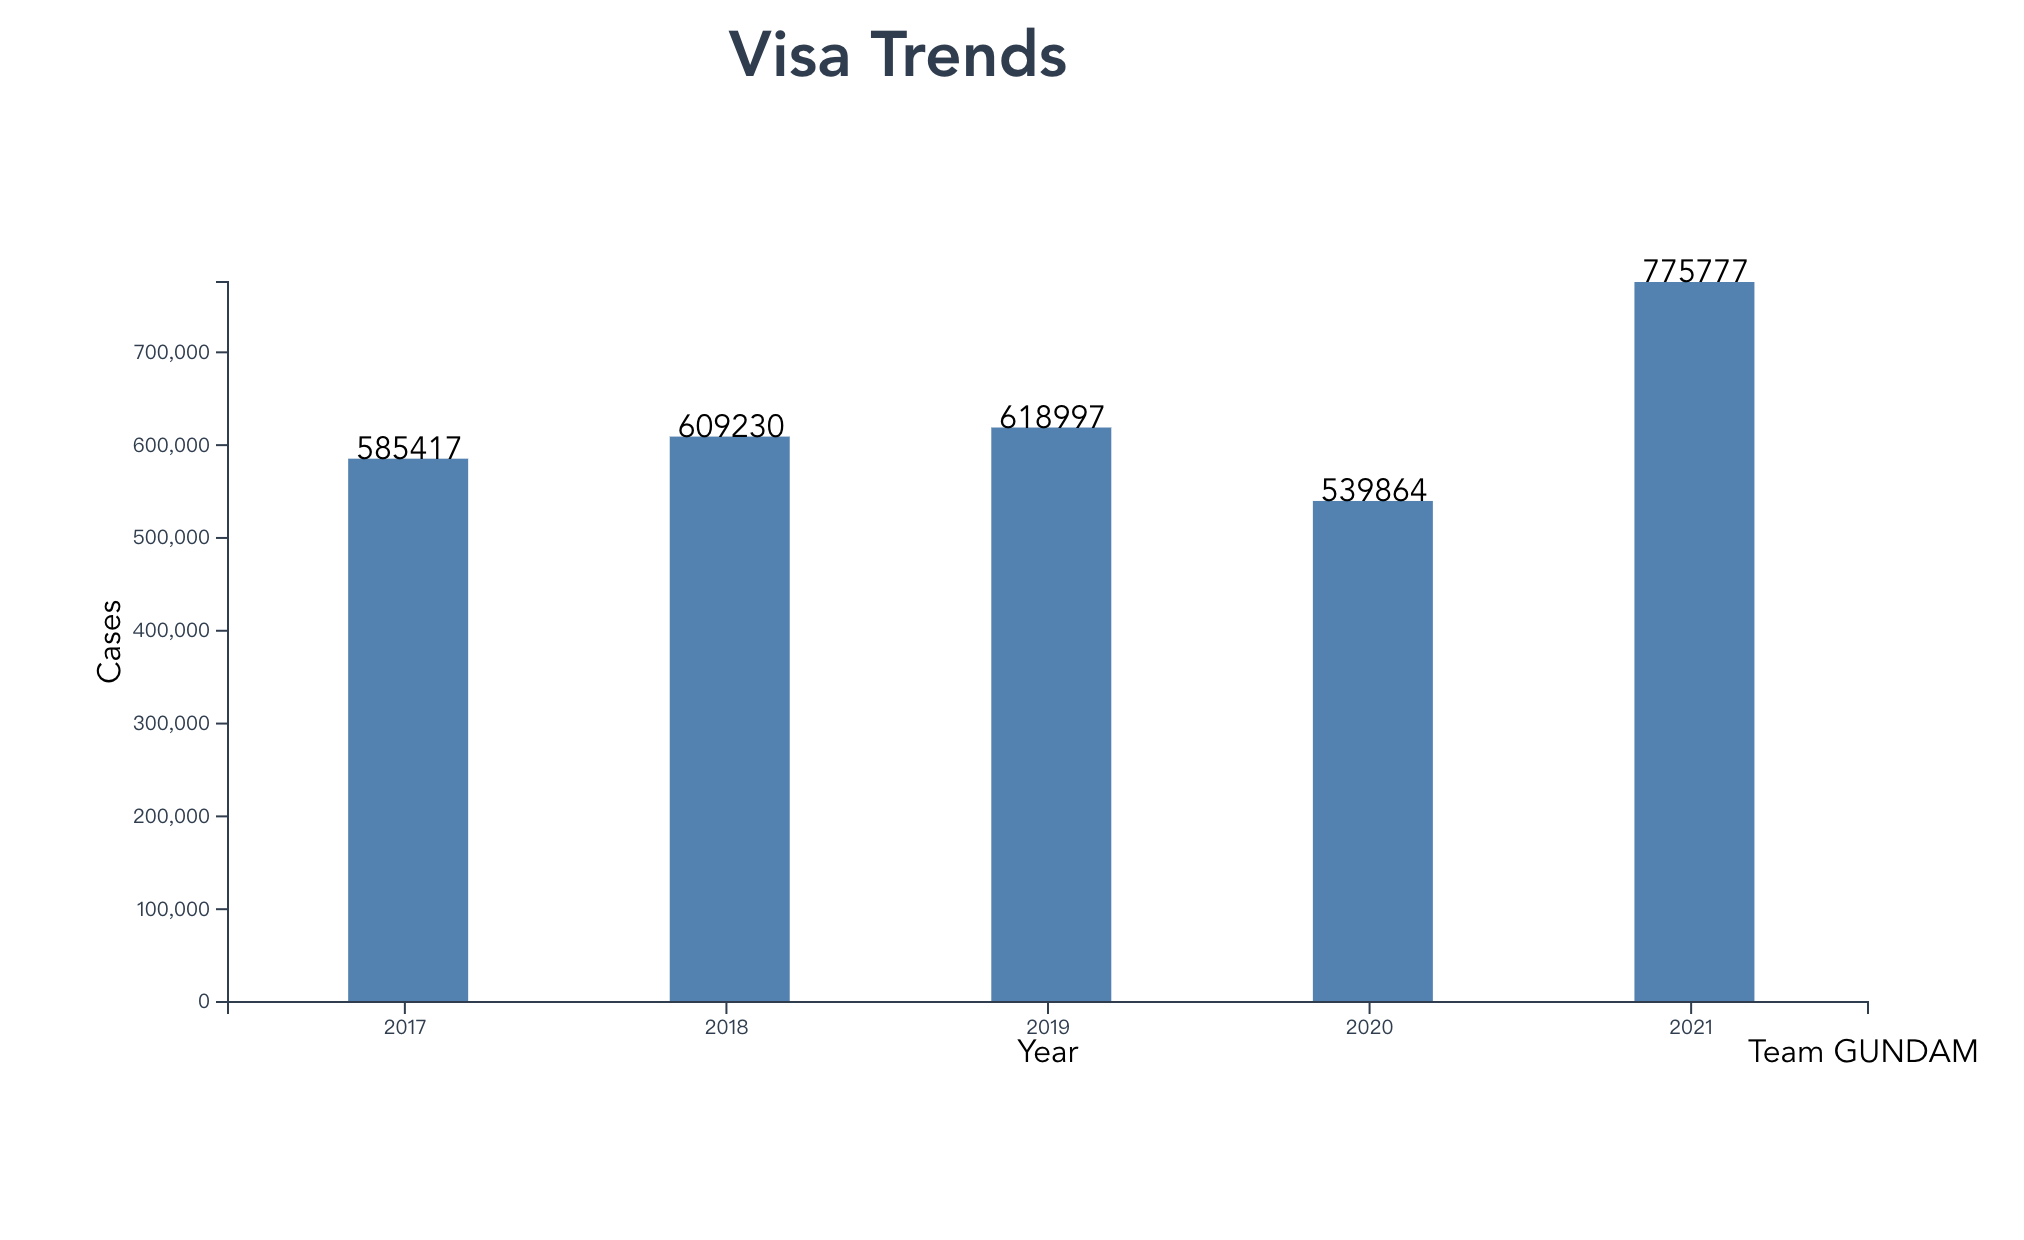
\includegraphics[width=\linewidth]{visa_trend.png}
%   \caption{Total Applications by Year}
%   \label{fig:appsbyyear}
% \end{figure}

\begin{figure}
  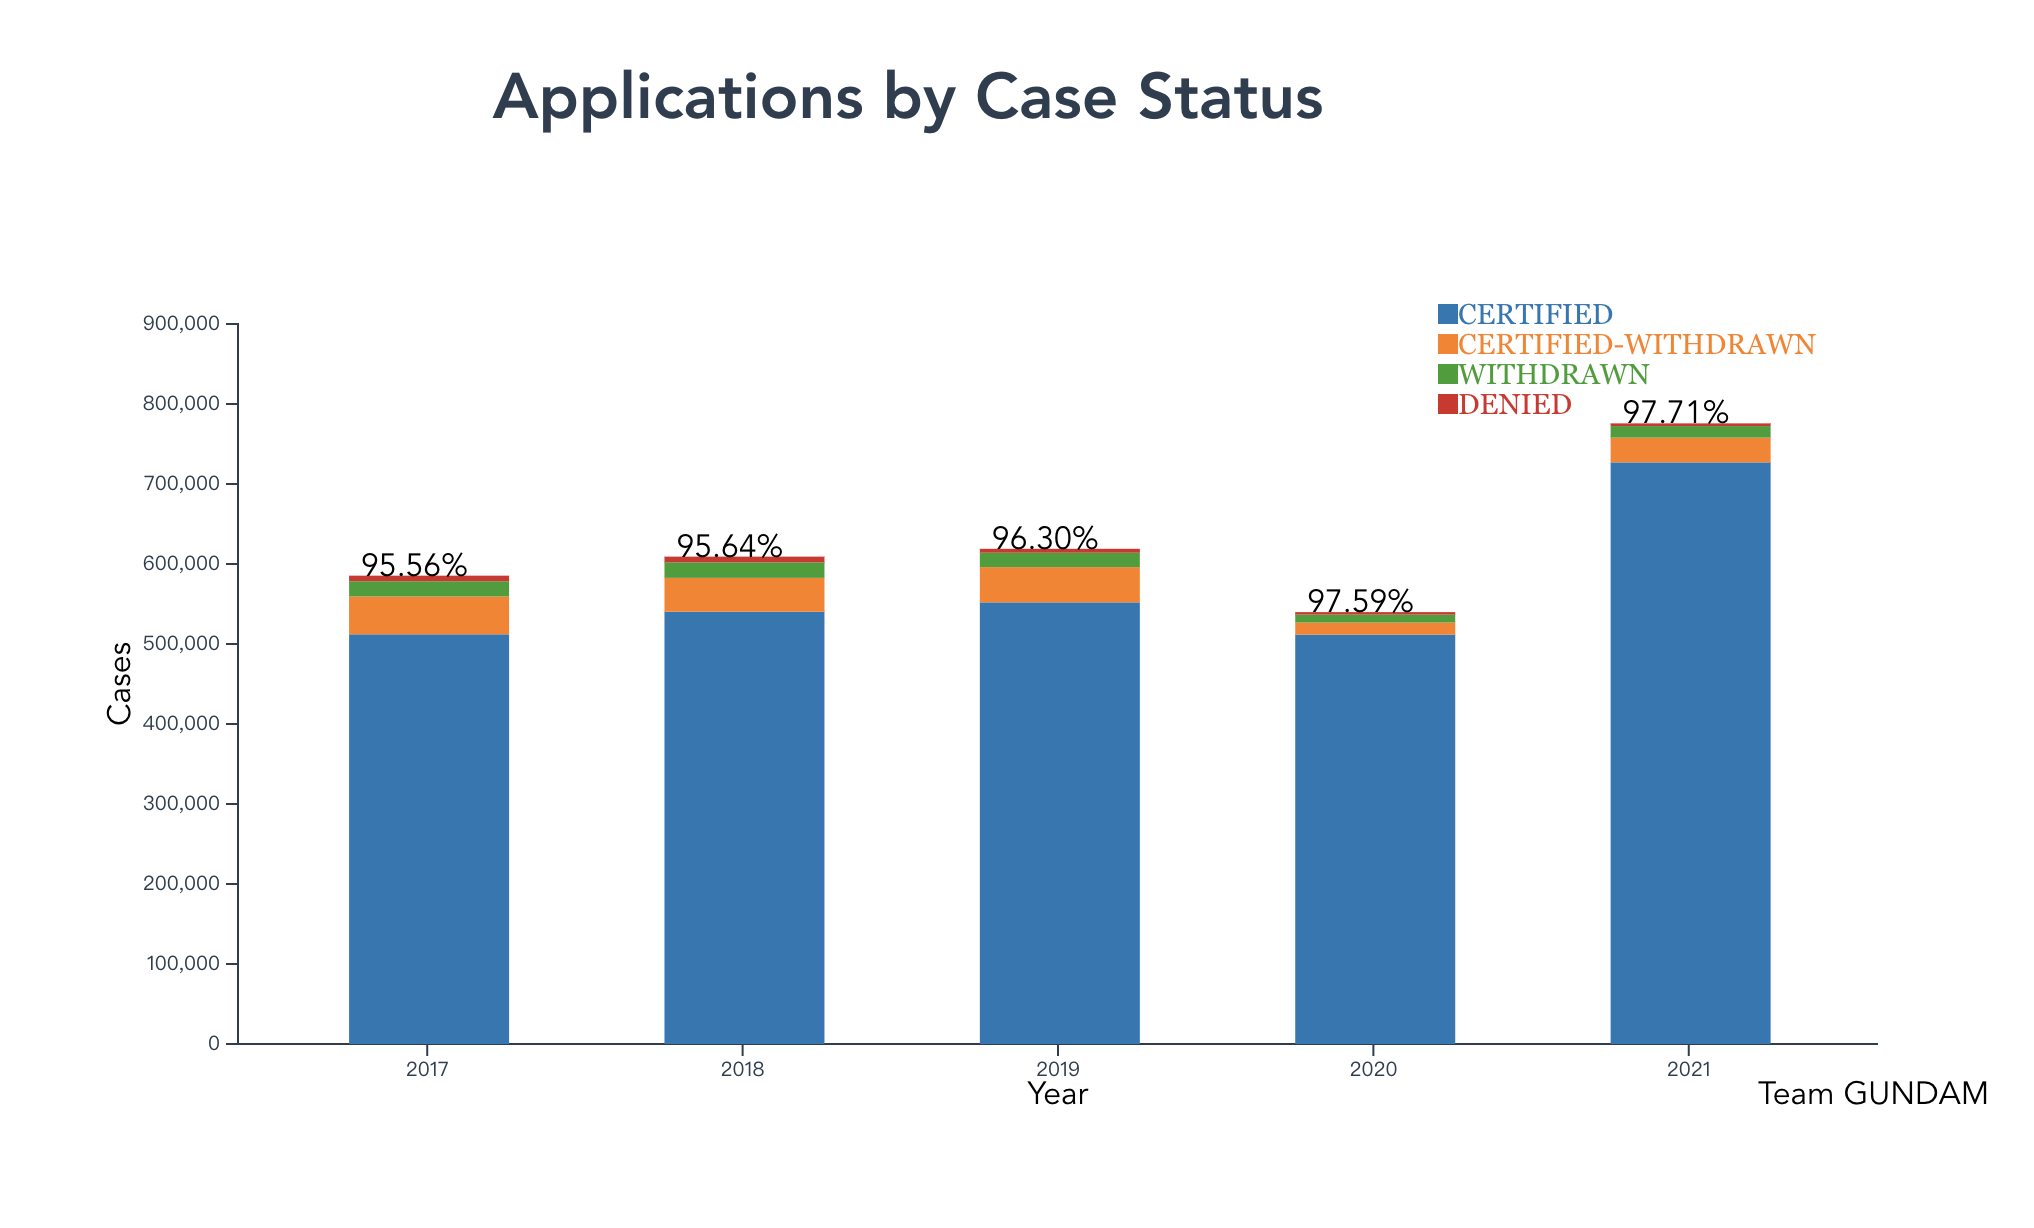
\includegraphics[width=\linewidth]{case_status_rate.png}
  \caption{Certifications by Year}
  \label{fig:casestatusrate}
\end{figure}

Naturally, the US choropleth map fits best for geographical comparison among states. To incrementally 
provide more information based on user feedback, we originally intended for each state to display a 
tooltip upon cursor hover, which includes key details such as the total applications for that year, the top employer, and the top 
job title. We were able to implement the tooltip in Javascript when embedded in HTML, but it would not display 
properly when integrated within the Vue framework. We instead include a dynamic table as a workaround, which updates with 
the above mentioned details in the same manner as a tooltip. 

We deploy our data analytics to provide an application certification prediction service, 
which takes user input parameters such as employer, job location, 
and expected salary, returning with over 95\% confidence the expected likelihood of 
such an application obtaining certification by the US Department of Labor. 
This is an exciting, new tool that allows the user to evaluate similar trends and relate these 
trends to their own individual situation. 
As the user inputs several keywords, suggestions are populated from which the user may select 
their desired employer and location. We hoped to include full elastic search supporting multiple 
user-defined parameters, but this proved to be beyond for the scope of this project. 

Although the overall volume of our data is quite large at roughly 450 MB, 
each individual record size is trivial after feature selection; thus, we 
were able to handle the processing and querying of these records through Pandas data frames, 
bypassing the need for a database. 




\begin{figure}
  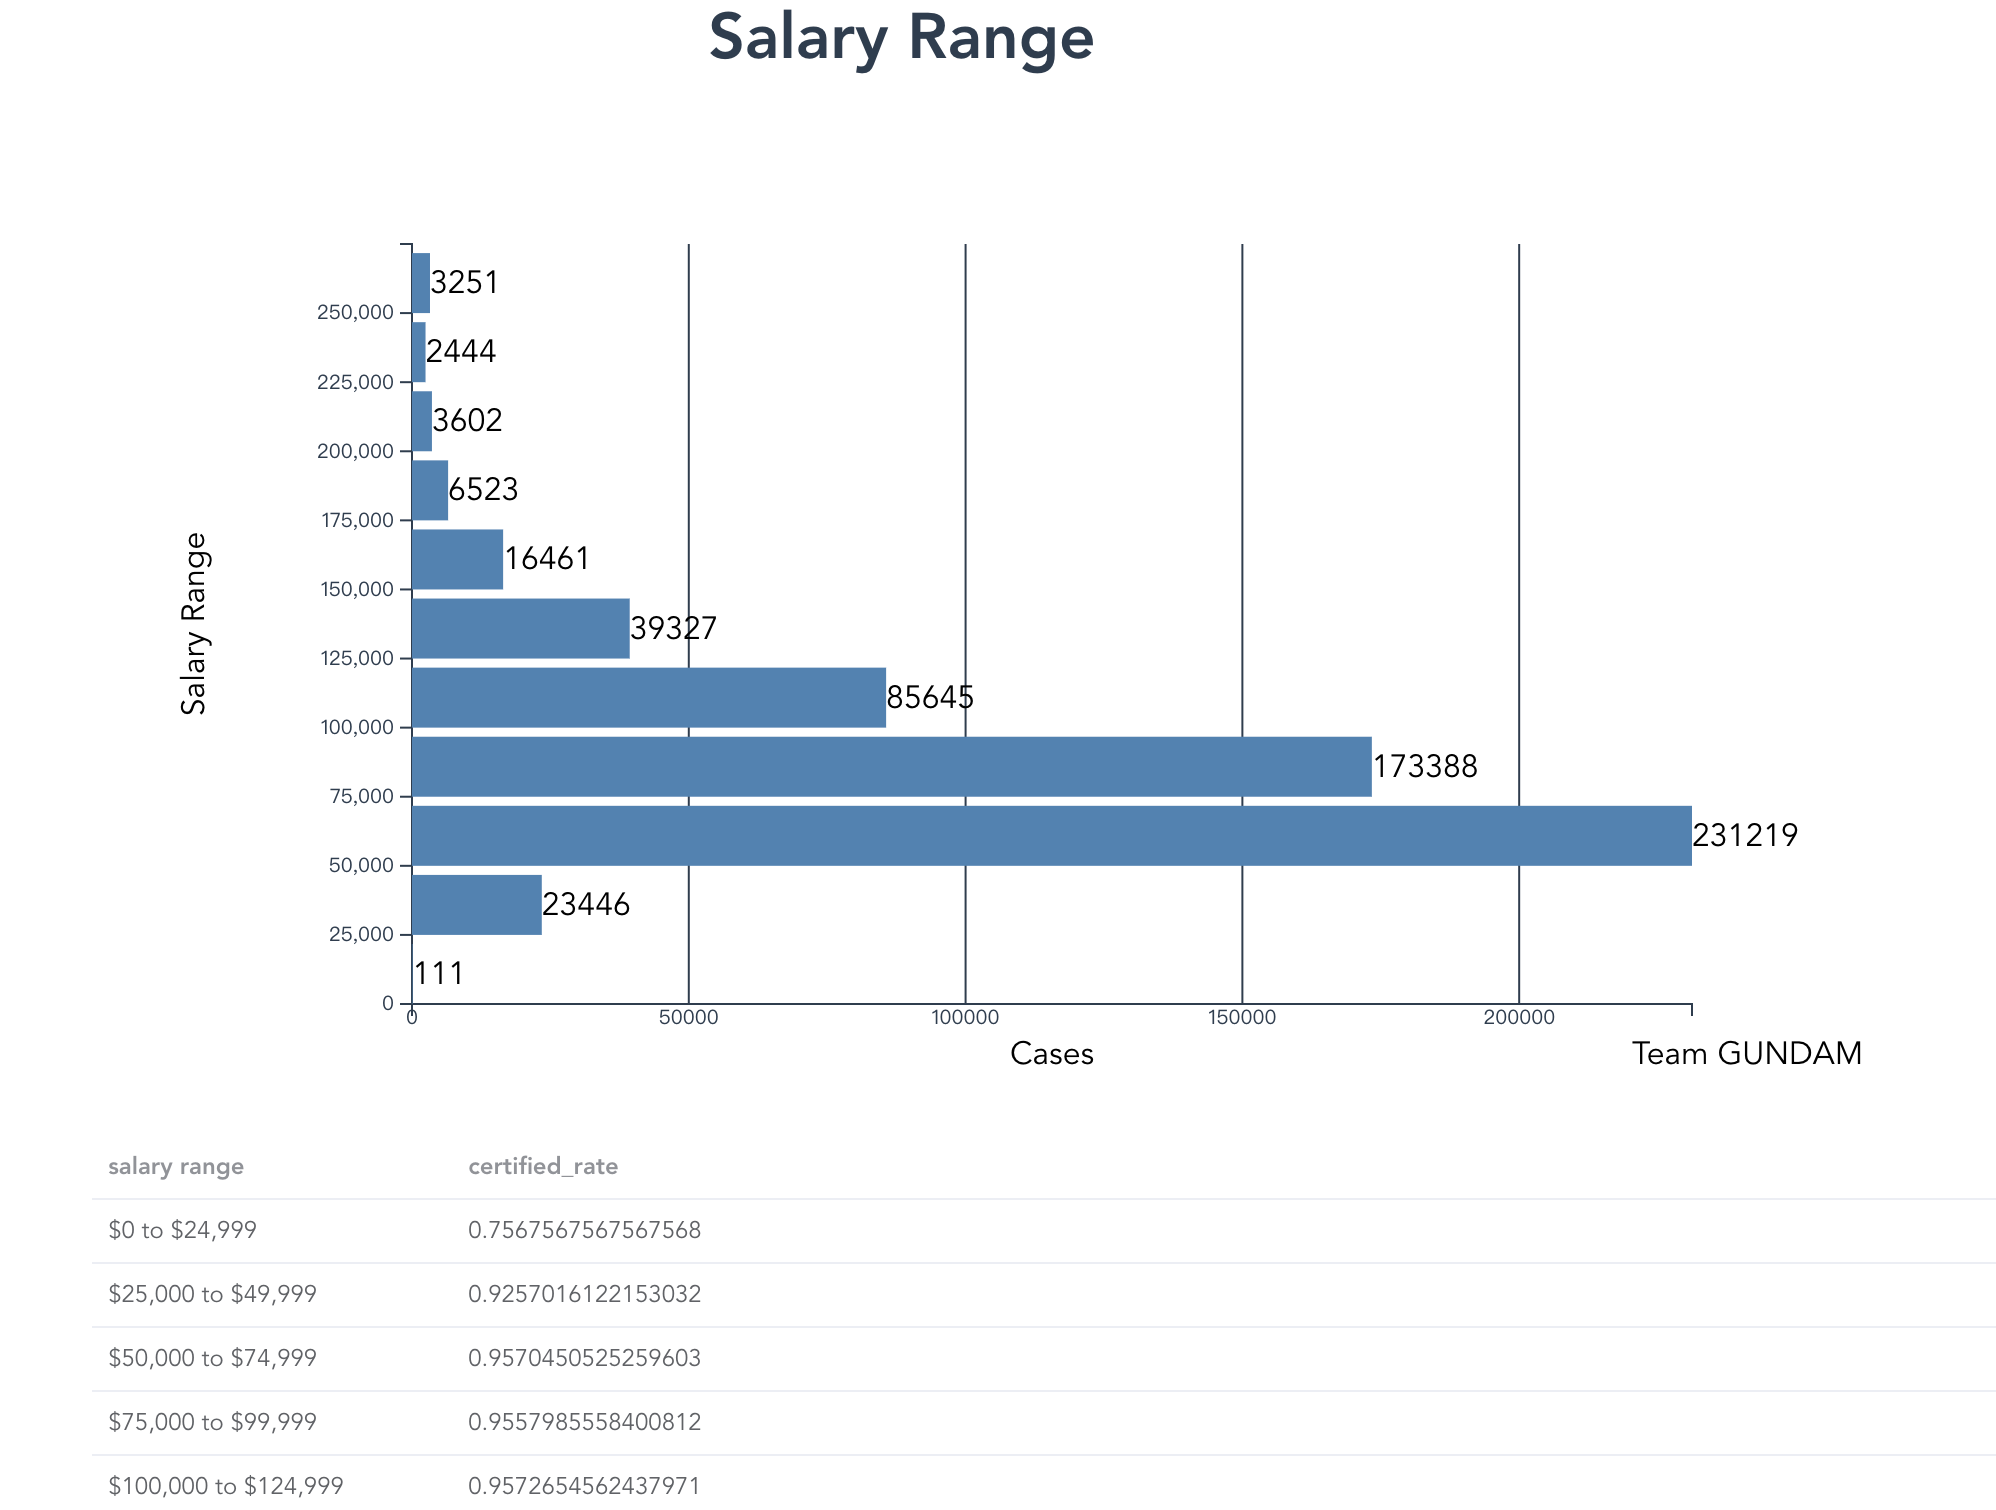
\includegraphics[width=\linewidth]{salary_range.png}
  \caption{Salary Range of Applications}
  \label{fig:salaryrange}
\end{figure}


\subsection{Analysis and Discussion}

% overall applications
The five-year period from 2017 and 2021 saw 32.52\% increase in overall H-1B applications, 
at an average of 6.50\% annual growth in applications, 
from 585,417 in 2017 to 775,555 in 2021. We witnessed a -12.78\% dip in 2020 - perhaps due to the 
uncertainty brought by COVID-19, including layoffs, hiring freezes, and travel restrictions 
enacted by several home countries of applicants, but 2021 saw a remarkable 43.70\% recovery in applications. 

The role of \textit{Software Developer, Applications} is by far the most popular job for applications, 
and continues to grow in popularity, ranging from 20.50\% to 28.90\% of total applications per year. 
Applications for this role alone grew 108.49\% in this five-year period,
 from 120,002 applications in 2017 to 250,192 in 2021, 
or three times faster than the overall number of H-1B applications received for all roles. 
All of the top five roles for each year are software development or computer systems related. 
This matches our expectations as the fastest growing companies in the US tend to be technology companies 
with a focus on software. 

California, Texas, and New York have the greatest concentration of overall applications 
for each of the five years observed in this study, which is understandable as 
these are also among the most populous US states. 
Interestingly, Florida, the third most populous state since 2018, is not among the 
top three states for certified applications. However, recent media discourse since 2021 
places Florida as a top destination for many large corporations seeking to relocate their major 
talent bases from New York, so we expect Florida to appear within the top five states within 
the next five years. 

\begin{figure}
  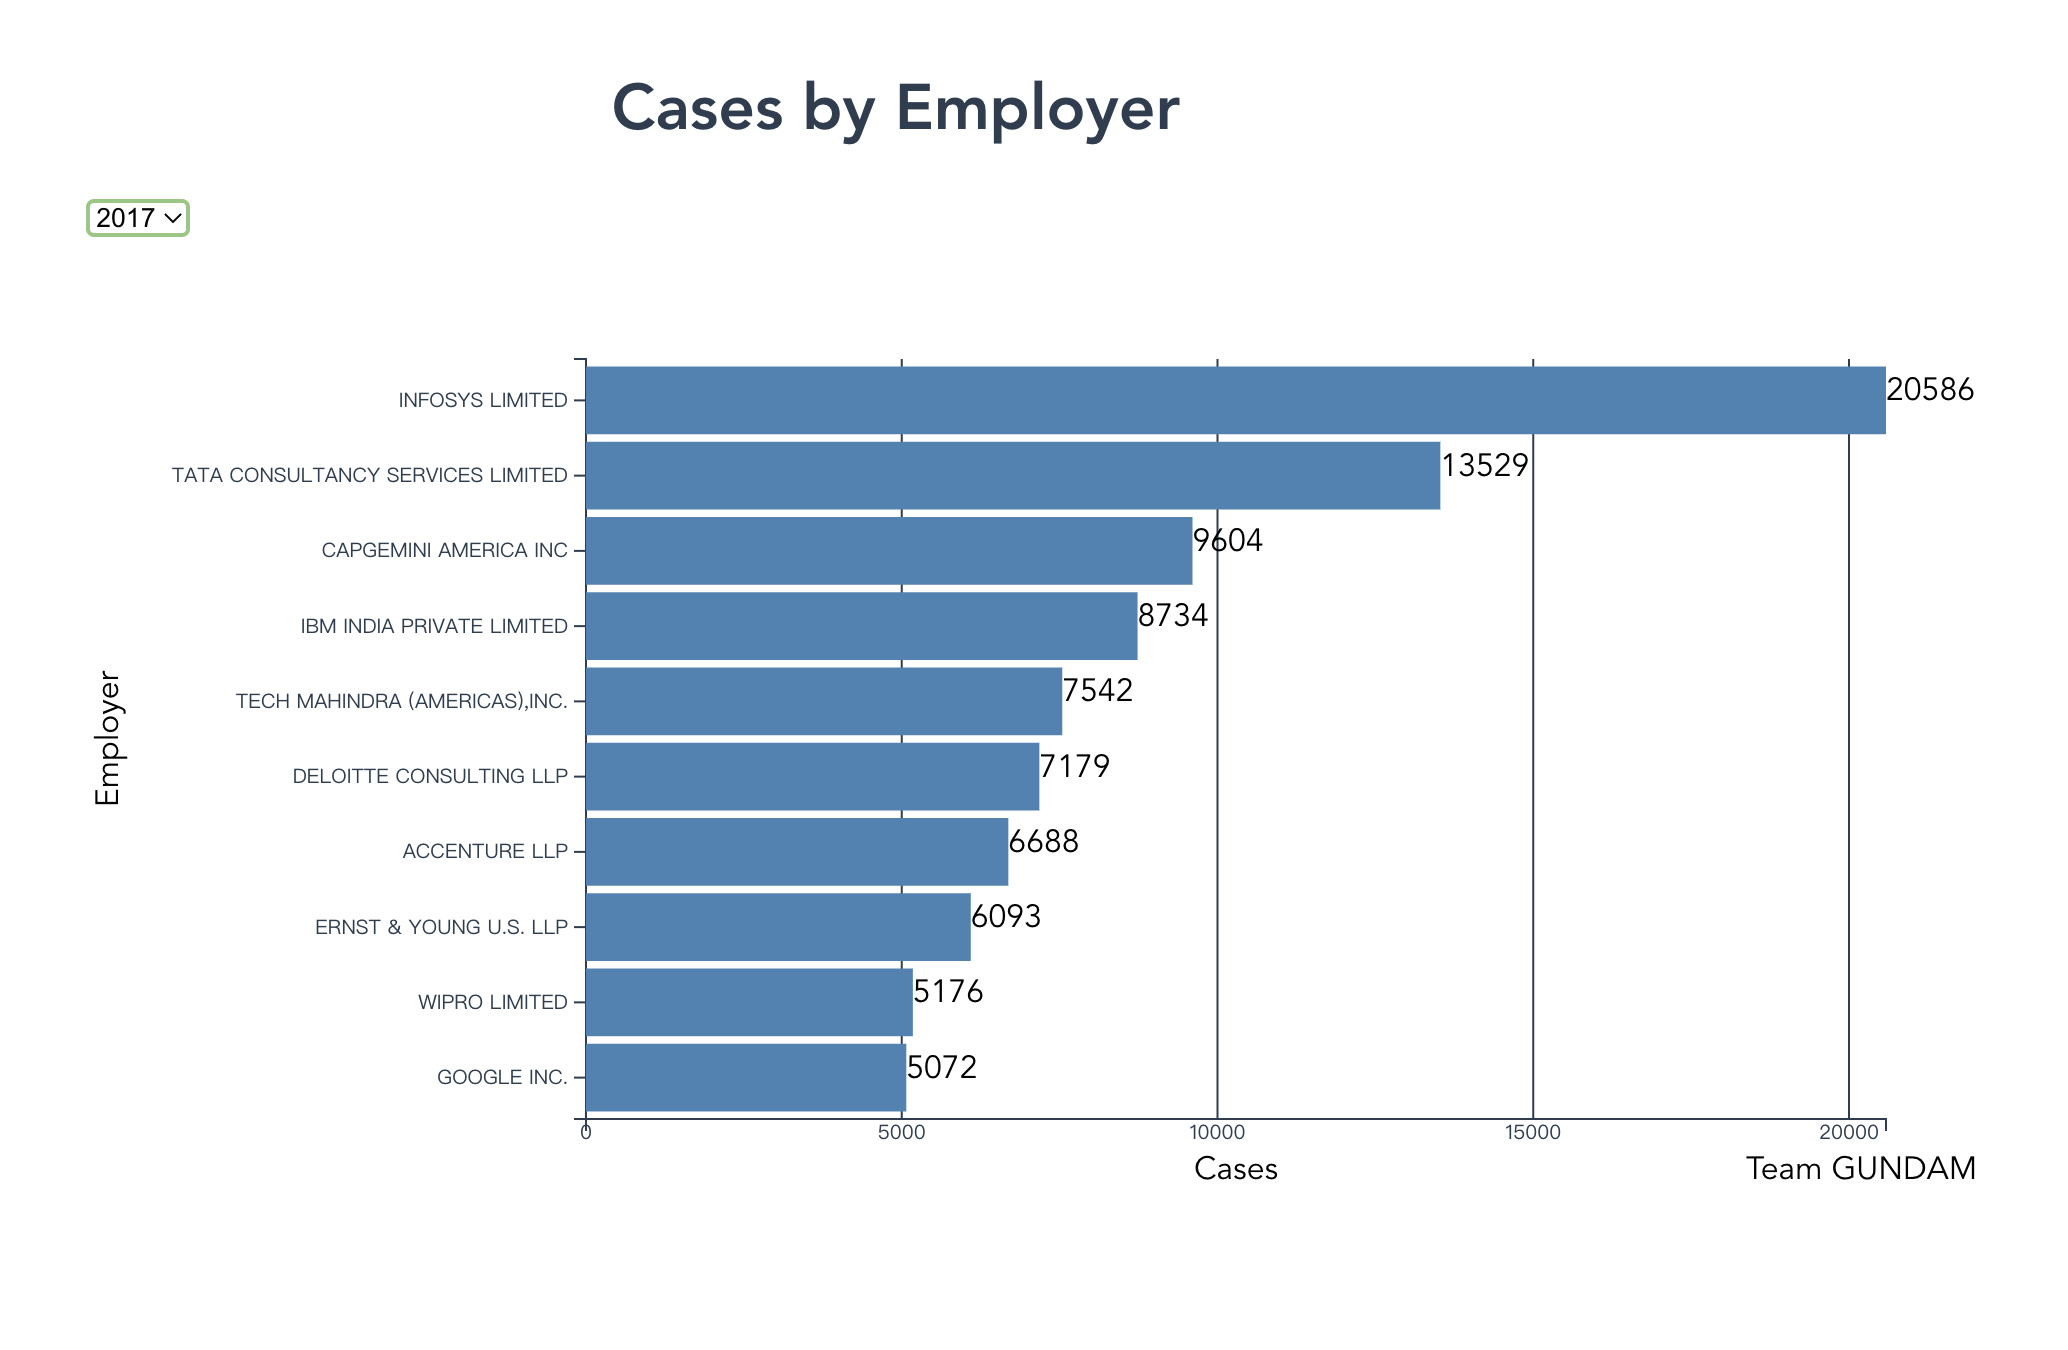
\includegraphics[width=\linewidth]{employer2017.png}
  \caption{Top 10 Employers by Applications - 2017}
  \label{fig:employer2017}
\end{figure}

\begin{figure}
  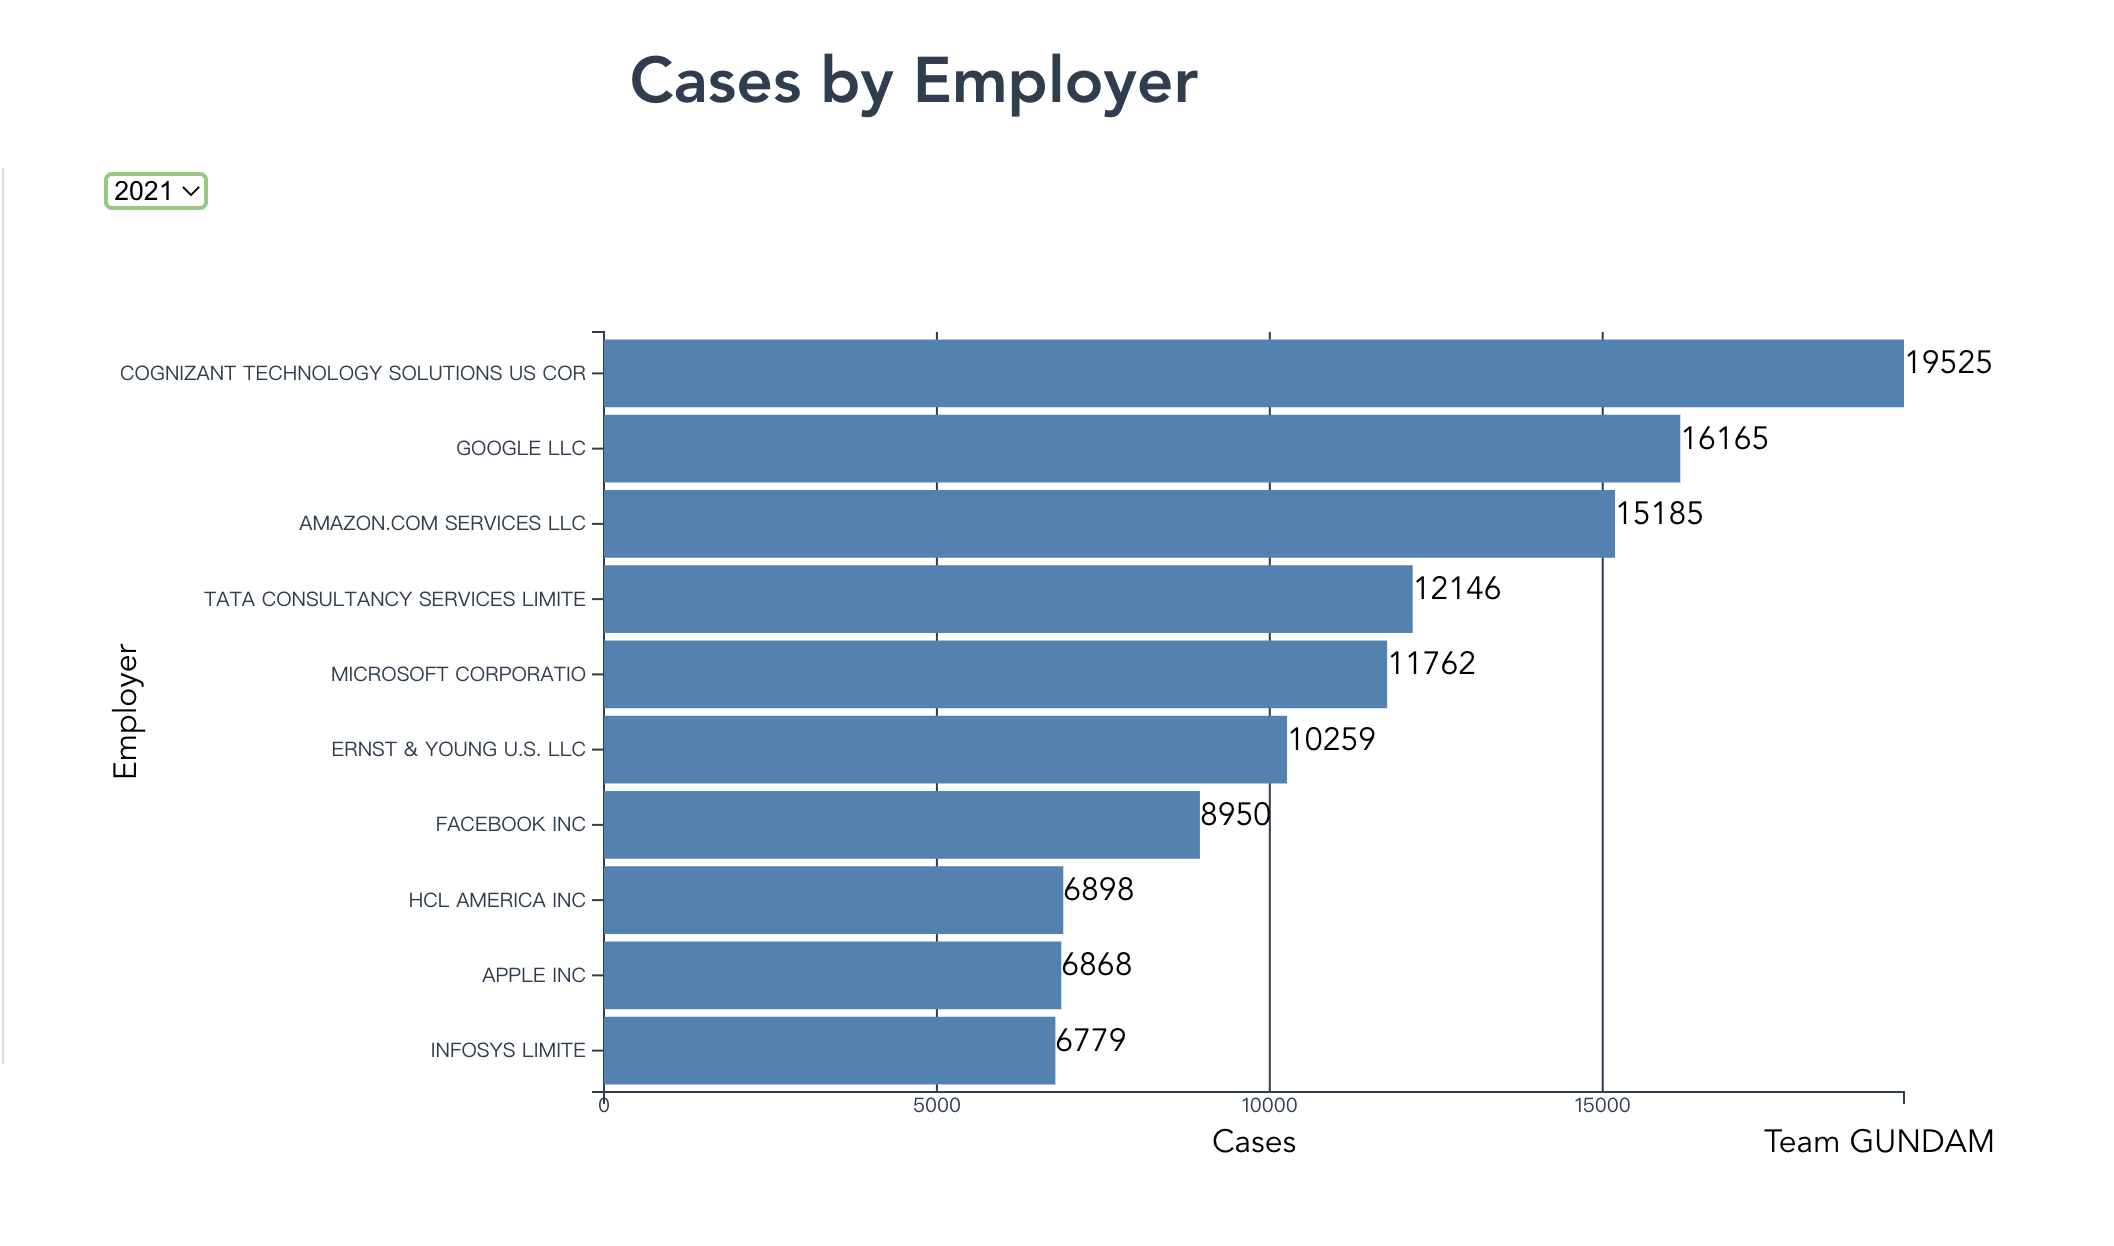
\includegraphics[width=\linewidth]{employer2021.png}
  \caption{Top 10 Employers by Applications - 2021}
  \label{fig:employer2021}
\end{figure}


The top ten employers in number of applications account for roughly 15\% of total applications each year. 
We see an interesting transition in the makeup of the top ten employers applying for the 
greatest number of visas during this period:
In 2017, the majority of these top ten companies are  
in IT consulting services - 9 in 2017 and 2018 - with their representation shrinking to 
7 in 2019 and 2020, and finally to 5 in 2021, with the largest US technology firms taking up more positions 
in the top ten. Although IT consulting services firms are not necessarily reducing annual applications, 
their growth is outpaced by 
% This change in the ordering of top employers can be attributed to 
% the consolidation of multinational IT consulting firms' US businesses, 
the immensely fast overall growth of US blue-chip technology firms such as Google, Amazon, and Facebook 
in recent years, leading to a major uptick in the direct hiring and sponsorship of foreign workers 
as a larger proportion compared to more traditional contracting practices. 


% The top job each year is Applications Software Developer. The number of applications 
% for this role grew at a 

Among the twelve attributes in our classifier model, we found the most influential attribute 
by far to be the employer sponsoring 
the application. This begs the question: What practices are these employers employing 
to hire the workers that most closely match US strategic interests? 
Is this the result of best-in-class hiring practices, or is it primarily due to 
recent trends and outpaced growth in selected industry verticals? 
Or is there encouragement to stimulate economic growth in certain geographic areas? 


Worksite city came in as a distant second with respect to the employer. 
With regards to location, the difference in significance between worksite city 
and worksite state is staggering, with worksite city showing six times more significance 
than the worksite state. This indicates that states themselves do not have an absolute advantage 
when it comes to application certification. One may argue that states hosting clusters of 
the more successful cities do indeed enjoy such hegemony, but our data is inconclusive in this regard.
Indeed, the metropolitan area of the company plays a much more important role than the state alone. 


As the initial premise for the H-1B program is to bring in qualified workers in specialty 
occupations with urgent 
talent needs, we expected industry and job title to play a more important role than 
the above two attributes. Their significance 
score are high; however, they place immediately after employer and worksite city. 


The remaining attributes ranged from having a small to negligible effect on the prediction results. 


\begin{figure}
  \begin{tabular}{ |p{4cm}||p{2cm}|  }
    \hline
    \multicolumn{2}{|c|}{\textbf{Feature Importance}} \\
    \hline
    Feature & Score\\
    \hline
    Employer Name & 1513.5\\
    Worksite City & 490.5\\
    NAICS Code & 319.9\\
    SOC Code & 240.4\\
    Wage Rate of Pay - From & 99.9\\
    Worksite State & 88.2\\
    Employer Business DBA & 82.6\\
    Prevailing Wage & 81.9\\
    Wage Unit of Pay & 32.9\\
    Prevailing Wage Unit of Pay & 24.6\\
    Total Workers & 22.2\\
    Full Time Position & 3.4\\
    \hline
   \end{tabular}
  \caption{Feature Importance}
   \label{fig:featureimportance}
\end{figure}


\section{Conclusion} 

Through the research conducted on H-1B visa application process, exploring the tools and technologies 
to process and extract information from the data, and experimenting with different media to 
express our findings, we have successfully applied the skills and leveraged the tools touched 
upon in class to devise a novel solution for a real need among international students. 
In an effort to quickly become proficient in this domain, we have also studied 
the intricacies of the US work visa application process, familiarizing ourselves 
with the geography and industry makeup of the United States. 

After discussion among our CSE 6242 peers, we have found several areas that require further 
improvement before we deploy our application to production. 
For multiple layer filtering of search criteria, although we successfully visualized the 
relevant data in an initial static representation, we have yet to implement a workaround 
in Vue to display the tooltip in our choropleth charts showing top employers 
and job titles for each state. In a future iteration, showing more granular statistics, 
such as the top jobs for each employer and the top states for each job, would add to 
the information value of each bar chart. 

Although over half of our total time spent on this project 
was cleaning and wrangling data, some inconsistencies remain. Rectifying these errors as well 
as special characteristics of other features will be a key focus in future improvements. 
The readability of aggregated employer statistics can be further improved by further exploring 
company name changes and parent company information. This would require collecting data from another 
source to serve as a reference for more advanced data wrangling. 

The reader should keep in mind that US DOL certification does not guarantee an 
applicant will receive a visa; 
rather, it only certifies that the 
position for which the applicant is hired meets the requirements. 
Certified applicants are then entered into a pool of 
applicants, from which the US Citizenship and Immigration Services randomly 
selects 65,000 initial applicants to receive 
the H-1B visa. Unsuccessful applicants holding a Master's degree or higher are 
then entered into a smaller pool from which 
20,000 applicants are selected. This step is essentially a lottery, 
primarily based on factors out of 
the applicant's control. Based on our research, serious applicants would most 
greatly benefit from understanding the 
qualities possessed by successful applicants at the top employers - those with 
the highest certification rate - and 
working towards that benchmark. Possessing a postgraduate degree would also 
significantly increase one's chances of 
acceptance by providing a second shot at one of the 20,000 slots exclusively 
for postgraduate degree holders. 


\begin{figure}
  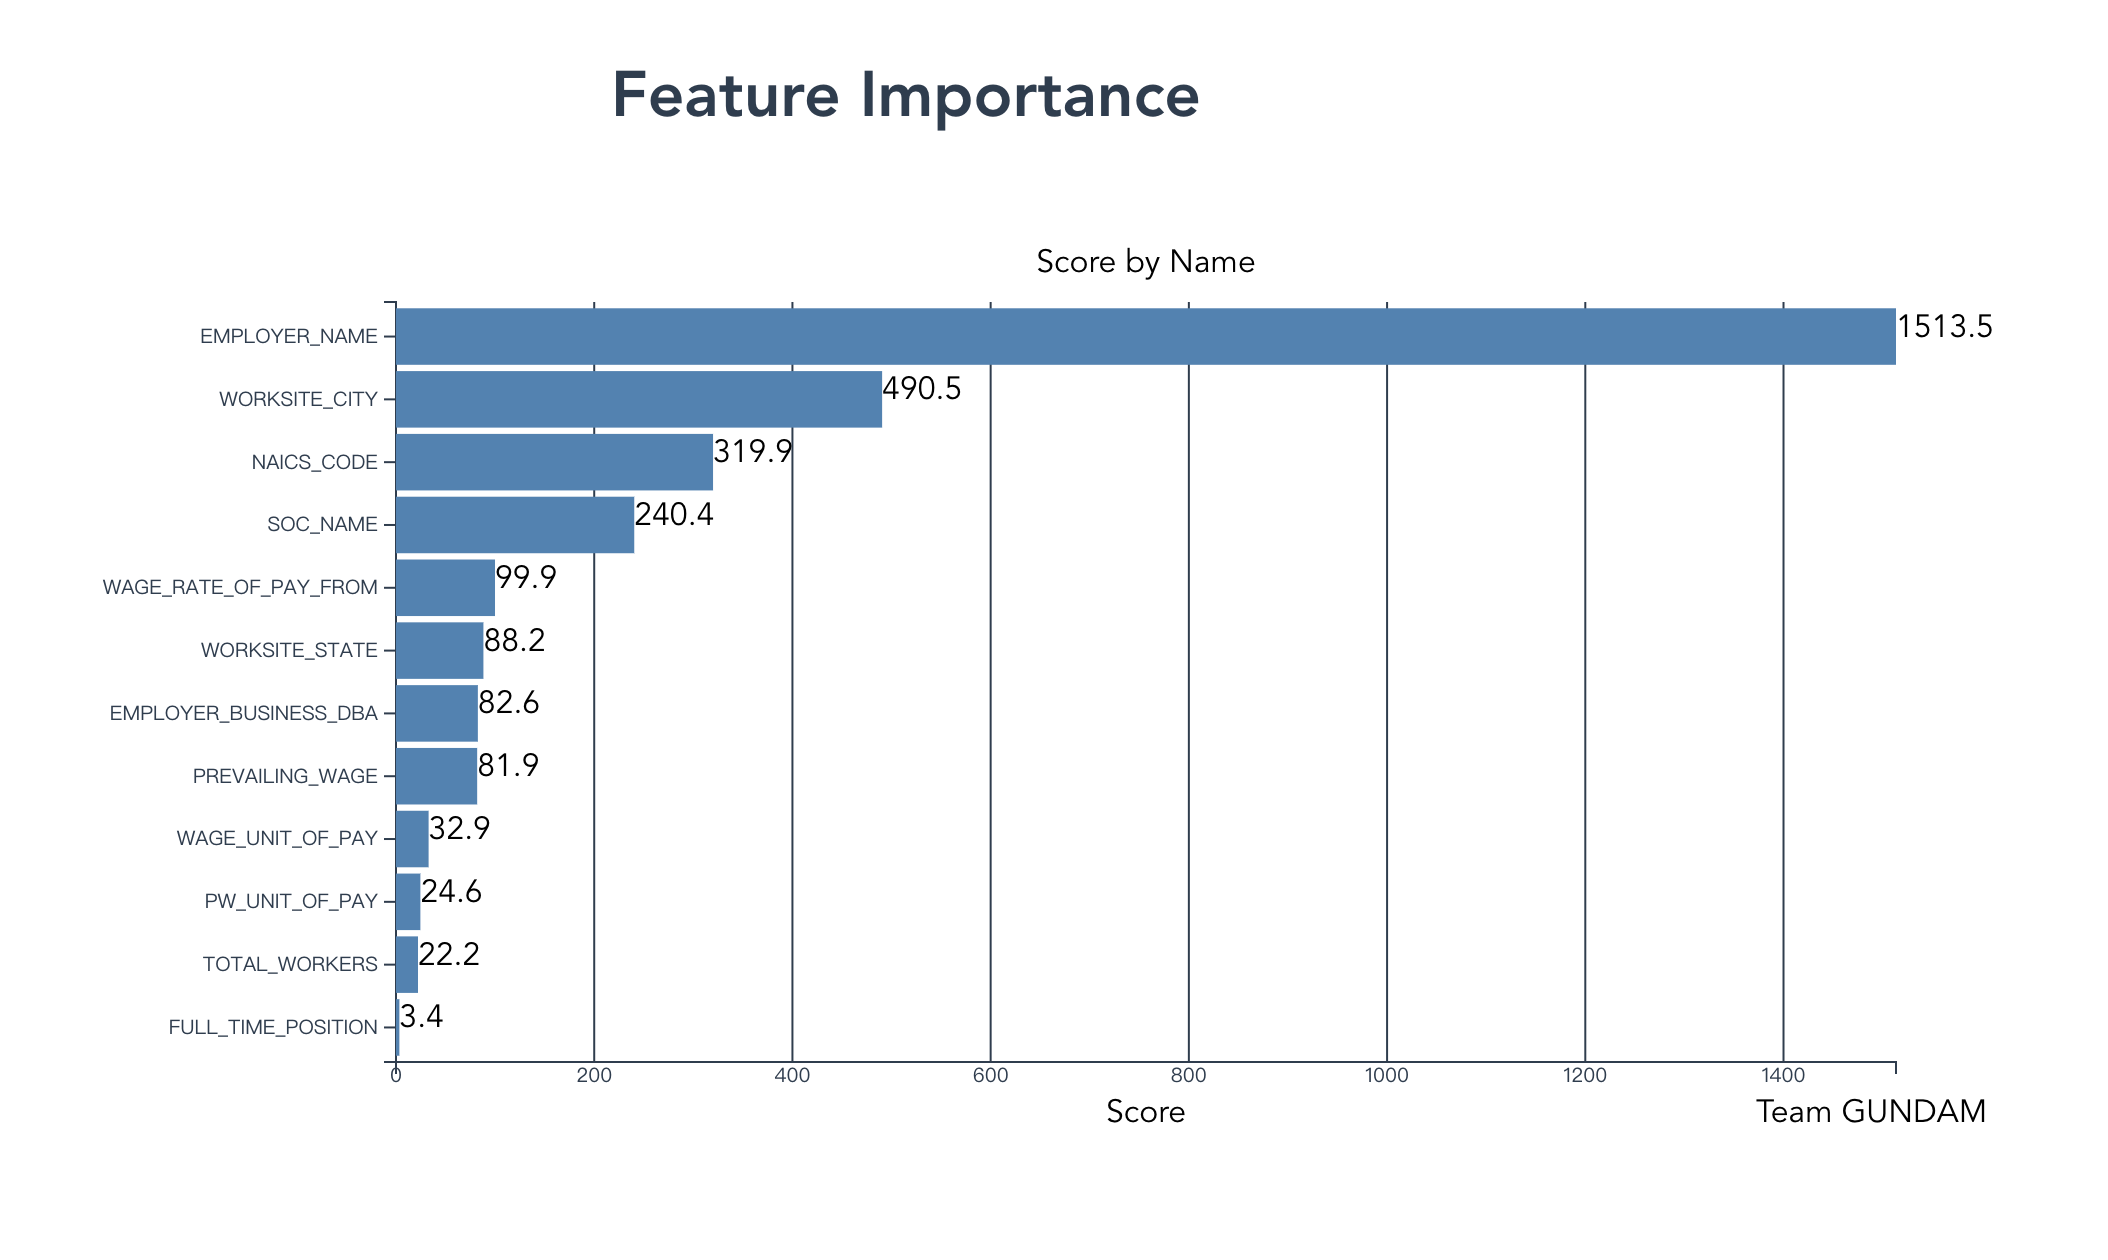
\includegraphics[width=\linewidth]{feature_imortance.png}
  \caption{Feature Importance}
  \label{fig:featureimportance}
\end{figure}


\appendix

\section{Work distribution}

Our team contributed a total of 136 hours to this study and its implementation. 




All team members have contributed similar amount of effort and results to this project.
 
\begin{itemize} 
	\item Project coordinator: Tianshu 
	\item Data collection, cleaning, wrangling, feature selection: Alexander, Tianyu, Chuanqi 
	\item ML algorithm design and implementation: Chuanqi 
	\item UI and visualization design: Alexander, Qinrui, Chuanqi, Tianshu, Tianyu
	\item Visualizations, frontend implementation: Tianshu, Tianyu 
	\item Data processing, backend implementation: Tianyu, Tianshu
	\item Documentation: Alexander, Qinrui, Chuanqi, Tianshu, Tianyu 
	
\end{itemize}
\begin{figure}
  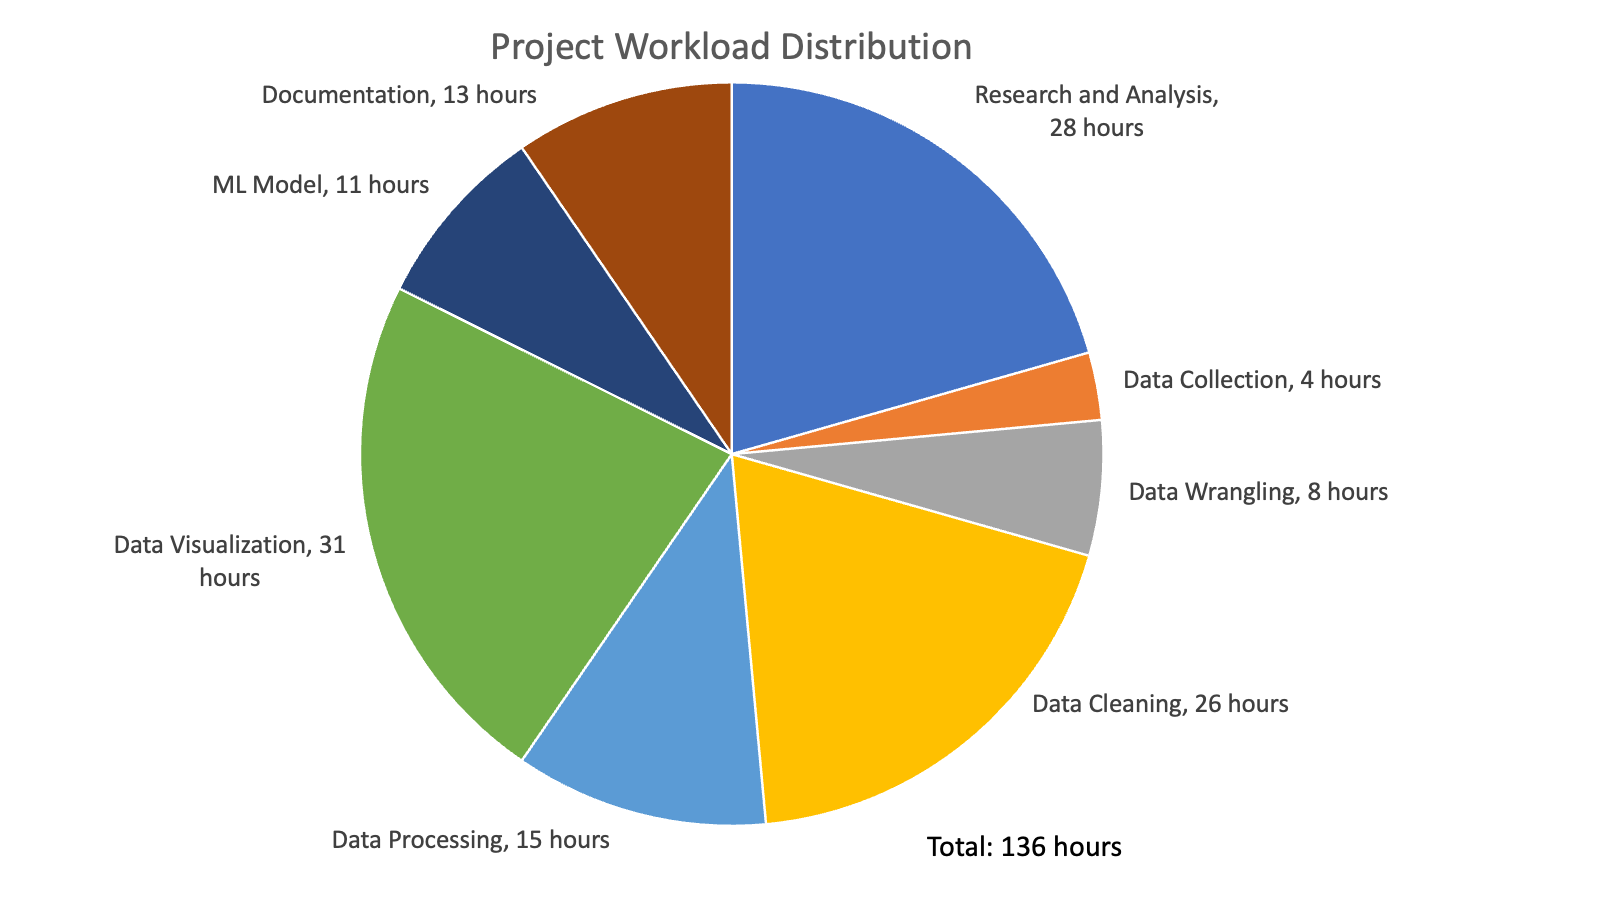
\includegraphics[width=\linewidth]{fig5_work_distribution.png}
  \caption{Work Distribution}
  \label{fig:workdistribution}
\end{figure}

\section{Innovations}
\begin{itemize}
	\item More selections and chart types that are more relevant to the user, such as a US choropleth with state-by-state comparison
	\item Ability to combine search parameters such as state and salary
	\item Interactive H-1B application outcome prediction through machine learning

\end{itemize}



\begin{thebibliography}{12}

\bibitem{}

\textit{}
Peri, G., Shih, K. Y., \& Sparber, C. 
(2014). 
Foreign STEM workers and native wages and employment in US cities (No. w20093). 
\textit{National Bureau of Economic Research. }
\url{https://www.nber.org/system/files/working_papers/w20093/w20093.pdf}.

\bibitem{}
Butler, E. W. 
(2012). 
The H-1B visa immigration program: Analysis and comments. 
\textit{International Journal of Business and Social Science, 3(9).}
\url{https://citeseerx.ist.psu.edu/viewdoc/download?doi=10.1.1.1066.7924&rep=rep1&type=pdf}.


\bibitem{}
Hermansen, A. S. 
(2022). 
Visualizing Intergenerational Immigrant Assimilation at Work. 
\textit{Socius,} 8, 23780231211072590.
\url{https://journals.sagepub.com/doi/full/10.1177/23780231211072590}.

\bibitem{}
Grimm, A. 
(2019). 
Studying to stay: Understanding graduate visa policy content and context in the United States and Australia. 
\textit{International Migration,} 57(5), 235-251. 
\url{https://ieeexplore.ieee.org/stamp/stamp.jsp?tp=&arnumber=9664747}.

\bibitem{} 
	H-1B Program. 
\textit{United States Department of Labor.} 
(2022). 
Retrieved 1 April 2022. 
\url{https://www.dol.gov/agencies/whd/immigration/h1b}.

\bibitem{}
Chatterjee, P., Velpuru, M. S., \& Jagadeeswari, T. 
(2021). 
Success of H-1B VISA Using ANN. 
\textit{In Machine Learning and Information Processing (pp. 491-499).}
 Springer, Singapore.

\bibitem{}
Thakur, P., Singh, M., Singh, H., \& Rana, P. S. 
(2018). 
An allotment of H1B work VISA in USA using machine learning. 
\textit{International Journal of Engineering \& Technology, 7(2.27), 93-103. }
\url{https://www.researchgate.net/profile/Prashant-Rana-4/publication/328488339_An_allotment_of_H1B_work_visa_in_USA_using_machine_learning}.

\bibitem{}
Dombe, A., Rewale, R., \& Swain, D. 
(2020). 
A deep learning-based approach for predicting the outcome of H-1B VISA application. 
\textit{In Machine Learning and Information Processing (pp. 193-202).}
 Springer, Singapore.

\bibitem{}
Visa Tracker - 1Point3Acres. 
(2022). 
Retrieved 1 April 2022.  
\\\url{https://visa.1point3acres.com/}.

\bibitem{}
H1B Database 2022 - Sponsors, Salaries, Approvals, Grades!. 
(2022). 
Retrieved 1 April 2022. 
\\\url{https://h1bgrader.com/}.

\bibitem{}
Tandon, A. 
(2021). 
ANALYSIS OF IMMIGRATION TRENDS IN THE US TO DISCOVER PATTERNS AND MAKE BETTER POLICY DECISIONS.
\\\url{https://scholarworks.lib.csusb.edu/cgi/viewcontent.cgi?article=2387}.

\bibitem{}
Tableau.
Retrieved 1 April 2022.
\\\url{https://tableau.com}.

\bibitem{}
CHAVDA, J. 
(2019). 
Big Data analysis on H-1B Visa Application in the United States.
\url{https://www.researchgate.net/profile/Jyoti-Chavda/publication/341132236_Big_Data_analysis_on_H-1B_Visa_Application_in_the_United_State/}.

\bibitem{}
Sundararaman, D., Pal, N., \& Misraa, A. K. 
(2017). 
An analysis of nonimmigrant work VISAs in the USA using machine learning. 
\textit{Int. J. Comput. Sci. Secur.(IJCSS), 6.}
\url{https://dhanasekar-s.github.io/research/3paper.pdf}.

\bibitem{}
Swain, D., Chakraborty, K., Dombe, A., Ashture, A., \& Valakunde, N. 
(2018, December). 
Prediction of H1B Visa Using Machine Learning Algorithms. 
\textit{In 2018 International Conference on Advanced Computation and Telecommunication (ICACAT) (pp. 1-7).} 
IEEE. 

\bibitem{}
Jethwani, G., Sachdeva, A., \& Goswami, M. 
(2019). 
An Empirical Analysis of ML Algorithms. 
\textit{Proceedings of International Conference on Sustainable Computing in Science, Technology and Management (SUSCOM),} 
Amity University Rajasthan, Jaipur-India.

\bibitem{}
Chadha, A. S., \& Shitole, A. 
(2021, November). 
A Hybrid Machine Learning Model Approach to H-1B Visa. 
\textit{2021 3rd International Conference on Electrical, Control and Instrumentation Engineering (ICECIE)} (pp. 1-8). 
IEEE.
\url{https://www.researchgate.net/publication/357663888_A_Hybrid_Machine_Learning_Model_Approach_to_H-1B_Visa}.

\bibitem{}
Roy, R. (2021). 
Data Analysis of H1B Visa Applications.

\bibitem{}
D3: Data Driven Documents. 
Retrieved 1 April 2022. 
\\\textit{https://d3js.org/.}

\bibitem{}
Vue. 
Retrieved 1 April 2022. 
\\\textit{https://vuejs.org/.}

\bibitem{}
Flask. 
Retrieved 1 April 2022. 
\\\textit{https://flask.palletsprojects.com/en/2.1.x/.}

\bibitem{}
OpenRefine. 
Retrieved 1 April 2022. 
\\textit{https://openrefine.org/.}

\bibitem{}
LightGBM. 
\textit{Microsoft.} 
Retrieved 1 April 2022. 
\\\textit{https://github.com/microsoft/LightGBM.}




\end{thebibliography}

\end{document}
